\section{Simhash-based Website Model}
\label{s:swm}
\subsection{Computation}

Here's a typical figure reference.  The figure is centered at the
top of the column.  It's scaled.  It's explicitly placed.  You'll
have to tweak the numbers to get what you want.\\

% you can also use the wonderful epsfig package...
\begin{figure}[t]
  \centering
  \begin{subfigure}
    \centering
    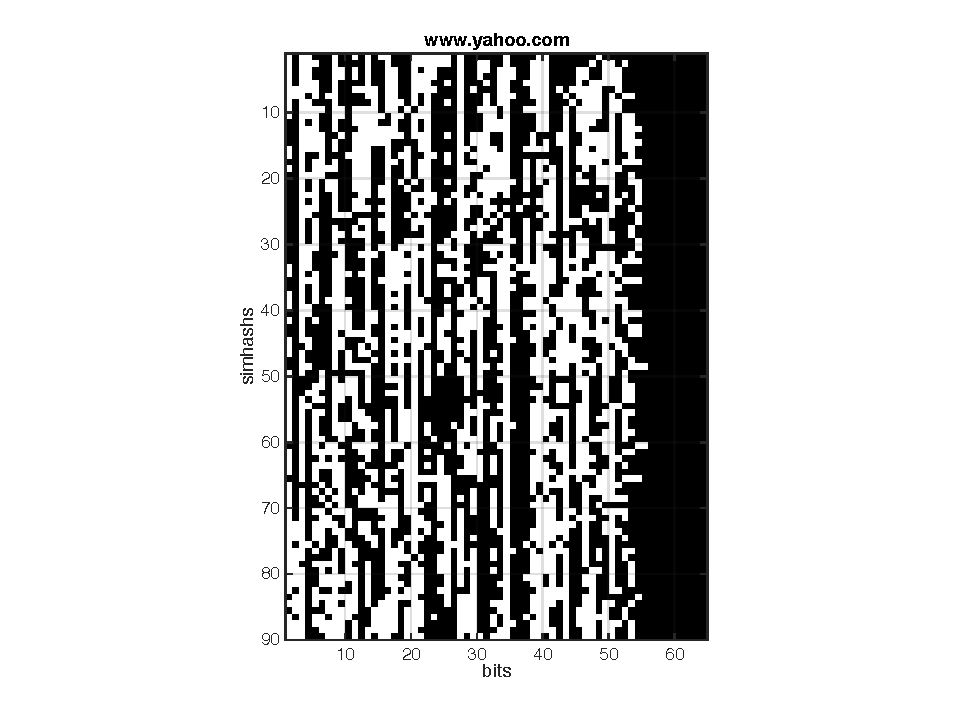
\includegraphics[width=.5\textwidth]{fig/yahoo-text}
    \label{fig:yahoo-text}
  \end{subfigure}%
  \begin{subfigure}
    \centering
    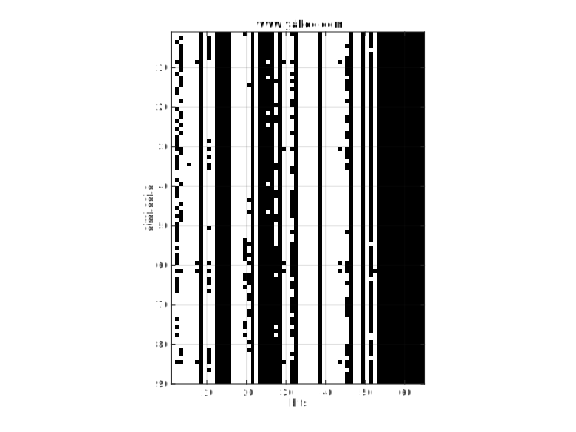
\includegraphics[width=.5\textwidth]{fig/yahoo-dom}
    \label{fig:yahoo-dom}
  \end{subfigure}
  \caption{Yahoo simhash changes over 7x24 period}
  \label{fig:yahoo-simhash}
\end{figure}


This text came after the figure, so we'll casually refer to Figure 1
as we go on our merry way.

\subsection{Aggregating / Clustering}

It can get tricky typesetting Tcl and C code in LaTeX because they share
a lot of mystical feelings about certain magic characters.  You
will have to do a lot of escaping to typeset curly braces and percent
signs, for example, like this:
``The {\tt \%module} directive
sets the name of the initialization function.  This is optional, but is
recommended if building a Tcl 7.5 module.
Everything inside the {\tt \%\{, \%\}}
block is copied directly into the output. allowing the inclusion of
header files and additional C code." \\

Sometimes you want to really call attention to a piece of text.  You
can center it in the column like this:
\begin{center}
  {\tt \_1008e614\_Vector\_p}
\end{center}
and people will really notice it.\\

\noindent
The noindent at the start of this paragraph makes it clear that it's
a continuation of the preceding text, not a new para in its own right.


Now this is an ingenious way to get a forced space.
{\tt Real~$*$} and {\tt double~$*$} are equivalent. 

Now here is another way to call attention to a line of code, but instead
of centering it, we noindent and bold it.\\

\noindent
{\bf \tt size\_t : fread ptr size nobj stream } \\

And here we have made an indented para like a definition tag (dt)
in HTML.  You don't need a surrounding list macro pair.
\begin{itemize}
  \item[]  {\tt fread} reads from {\tt stream} into the array {\tt ptr} at
    most {\tt nobj} objects of size {\tt size}.   {\tt fread} returns
    the number of objects read. 
\end{itemize}
This concludes the definitions tag.

\subsection{Model Selection}


\begin{table*}[!th]                                                     
  \centering                                                            
  \scriptsize                                                           
  \begin{tabular}{lllllllllll}
  \toprule
  & \multicolumn{2}{c}{\textbf{Normal}}
  & \multicolumn{2}{c}{\textbf{Lognormal}}
  & \multicolumn{2}{c}{\textbf{Exponential}}
  & \multicolumn{2}{c}{\textbf{Gamma}}
  & \multicolumn{2}{c}{\textbf{Logistic}}\\

  \textbf{Website(Hash Type)\textbackslash Model}
  & AD-value
  & P-value
  & AD-value
  & P-value
  & AD-value
  & P-value
  & AD-value
  & P-value
  & AD-value
  & P-value \\
  \midrule
  digg.com T & 0.617 &  0.100 & 0.481 &  0.219 &
  14.851 & < 0.003 & 0.538 &  0.186 & 0.531 &  0.131\\ 
  digg.com T & 0.227 &  0.806 & 0.179 &  0.914 &
  19.690 &  < 0.003 & 0.198 &  > 0.250 & 0.250 & >0.250\\
  yahoo.com T & 0.192 &  0.893 & 0.263 &  0.692 &
  35.828 & <0.003 &   0.231 & >0.250 & 0.222 & >0.250\\
  amazon.com T & 0.720 &  0.058 & 0.323 &  0.520 & 
  27.754 & <0.003 &  0.436 & >0.250 & 0.642 &  0.058\\
  reddit.com T & 0.373 &  0.411 & 0.331  & 0.509 & 
  35.063 & <0.003 & 0.340 & >0.250 & 0.361 & >0.250\\
  yacombinator.com T & 0.473 &  0.237 & 0.516 &  0.186 &
  37.551 & <0.003 & 0.519 &  0.204 & 0.583 &  0.089\\

  digg.com D & 0.319 &  0.372 & 0.348 &  0.305 &
  1.491 &  0.021 &  0.402 & >0.250 & 0.363 & >0.250\\
  yahoo.com D & 0.531 &  0.168 & 0.392 &  0.366 &
  18.837 & <0.003 & 0.441 & >0.250 & 0.584  & 0.088\\
  amazon.com D & 1.519 & <0.005 & 0.916 &  0.019 &
  22.083 & <0.003 & 1.052 &  0.009 & 0.548 &  0.114\\
  amazon.com D & 0.483 & 0.117 &  0.504 & 0.104 &
  1.741 & 0.010 & 0.601 & 0.128 & 0.523 & 0.115\\

\end{tabular}

                                     
  \caption{Model statistics for selected websites}
  \label{tbl:para-select}                                         
\end{table*}                                                            


This table ~\autoref{tbl:para-select} shows the Anderson-Darling (AD) value and P-value for each model.
A common rule used in model selection is pick the model which has the smallest
value with P-value greater than 5\%. Each row in the table represents one
website. From the statistics of these websites, we choose normal distribution
for text simhash and Lognomal distribution for dom simhash.

In the simhash based cloaking detection model, input from the user is simply simhash. How to compare against the simhashs that is already collected?

One simple way is to compute the average distance from this simhash to all the observed simhashs. The next step is then to tell whether this distance is reasonable. 

The text distribution follows lognormal distribution.
After mannual check of those results.




You have to run {\tt latex} once to prepare your references for
munging.  Then run {\tt bibtex} to build your bibliography metadata.
Then run {\tt latex} twice to ensure all references have been resolved.
If your source file is called {\tt usenixTemplate.tex} and your {\tt
bibtex} file is called {\tt usenixTemplate.bib}, here's what you do:
{\tt \small
  \begin{verbatim}
  latex usenixTemplate
  bibtex usenixTemplate
  latex usenixTemplate
  latex usenixTemplate
  \end{verbatim}
}


